\section{Results}

Each model is summarised through its drift matrix by the in-distribution, forward, and decay scores of \cref{subsec:drift_summary}, namely its performance on the period it was trained through, its mean performance on the later periods held out from training, and the difference between the two. How far a model degrades between them is governed by two factors that recur across the three domains, the strength of its inductive bias and whether it relies on a frozen pretrained encoder.

\begin{figure*}[t]
\centering
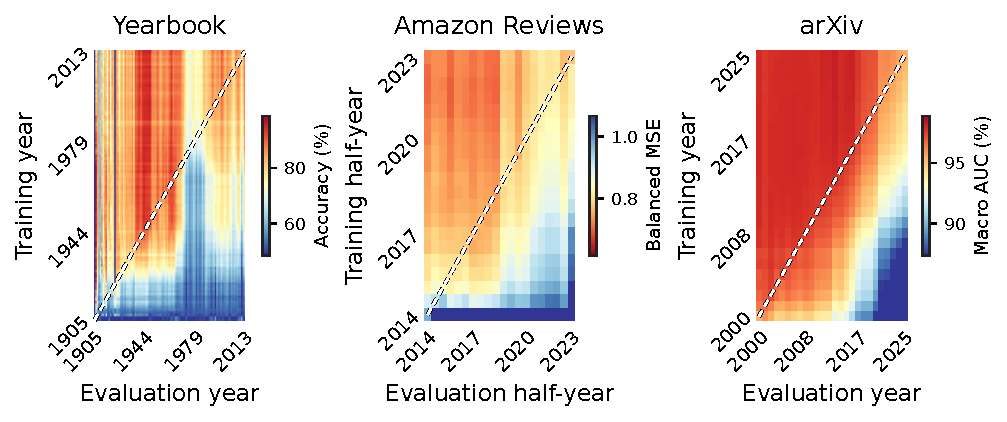
\includegraphics[width=\textwidth]{plots_experiments/combined/mean_matrices.pdf}
\iflncs
\caption{Cohort-mean drift matrices, one panel per domain. Each cell $(i,j)$ is mean performance across models when trained through period $i$ (row) and evaluated on period $j$ (column): accuracy for \texttt{Yearbook}, balanced MSE for \texttt{Amazon Reviews} (lower is better), and macro AUC for \texttt{arXiv}. The dashed diagonal marks in-distribution evaluation; the lower-right region is forward generalization. Vertical white bands mark periods with insufficient samples.}
\else
\caption{Cohort-mean drift matrices, one panel per domain. Each cell $(i,j)$ is the mean performance across all models of that dataset when trained on data through period $i$ (row) and evaluated on period $j$ (column): accuracy for \texttt{Yearbook}, balanced MSE for \texttt{Amazon Reviews} (lower is better), and macro AUC for \texttt{arXiv}. The dashed diagonal marks in-distribution evaluation; the lower-right region of each panel is forward generalization to unseen future periods. Vertical white bands mark periods with insufficient samples.}
\fi
\label{fig:mean_matrices}
\end{figure*}

\subsection{Image Classification}

On \texttt{Yearbook}, the model families separate sharply in distribution, along the diagonal of the cohort-mean matrix in the \texttt{Yearbook} panel of \cref{fig:mean_matrices}. MLP-S, which flattens the image into a vector and imposes no spatial structure, sits at about $\val{yearbook/model/mlp_s/indist}\%$, while the CNNs and ResNets reach near $\val{yearbook/model/cnn_l/indist}\%$ for CNN-M and CNN-L (\cref{tab:robustness_yearbook}). What sets these apart is their inductive bias toward locality and translation equivariance, by which they build features from small local regions of the image and recognise a pattern wherever it appears, and this lets them exploit the cues that most sharply separate male from female portraits within a given period. The ViTs and frozen encoders fall between these two ends.

Temporal robustness reverses this ordering, and we read it from the decay, the accuracy a model loses once the evaluation year moves past its training cutoff (\cref{tab:robustness_yearbook}). The CNNs and ResNets, strongest in distribution, decay the most, by $\val{yearbook/model/cnn_l/decay}$ and $\val{yearbook/model/cnn_m/decay}$ points for CNN-L and CNN-M, so their accuracy on future years falls to about $\val{yearbook/model/cnn_l/future}\%$. MLP-S is the steadiest model of all, with only $\val{yearbook/model/mlp_s/decay}$ points of decay, though from its lower starting accuracy of $\val{yearbook/model/mlp_s/future}\%$. The frozen pretrained encoders form a third group, more stable than the CNNs but less accurate to begin with, decaying by $\val{yearbook/frozen/decay-min}$ to $\val{yearbook/frozen/decay-max}$ points, with the self-supervised DINOv3-S steadiest among them and the supervised ImageNet-21k backbone least.

% Single-column LNCS: a normal figure places inline (avoids the top-float
% whitespace a double-column figure* strands); the two-column preprint keeps
% figure* so the wide grid spans both columns.
\iflncs\begin{figure}[htbp]\else\begin{figure*}[htbp]\fi
\centering
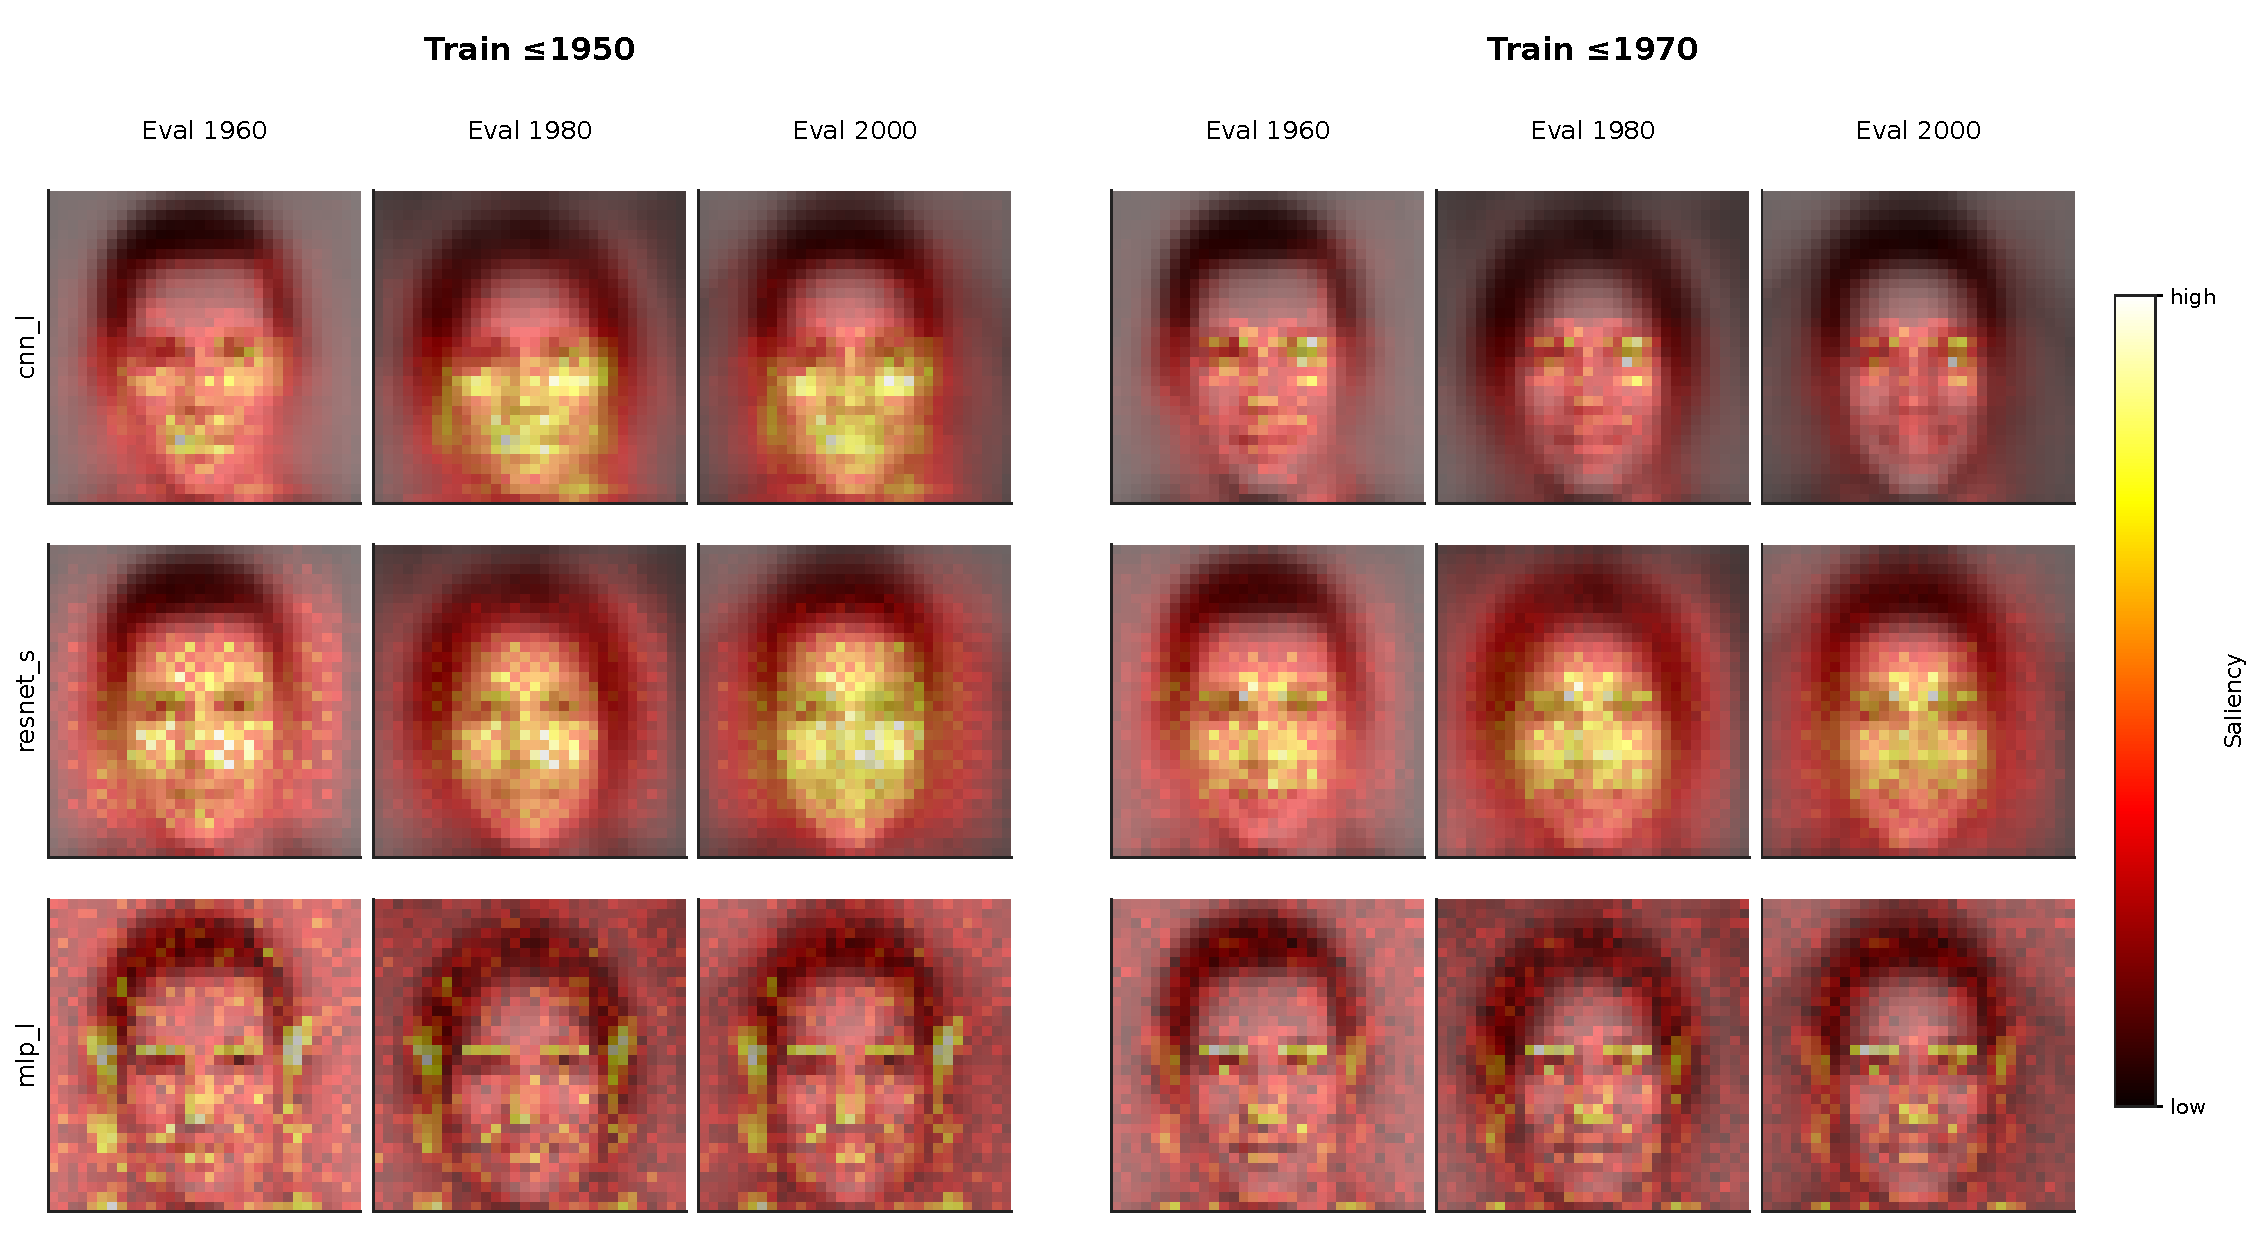
\includegraphics[width=\linewidth]{img/drift_matrices/saliency_cnn_resnet_mlp.pdf}
\caption{Gradient saliency maps on \texttt{Yearbook} for CNN-L, ResNet-S, and MLP-L, each trained through 1950 (left) and 1970 (right) and evaluated on later years. Each panel averages gradient saliency over the selected portraits from the indicated evaluation year rather than a single example.}
\label{fig:saliency}
\iflncs\end{figure}\else\end{figure*}\fi

What lifts a model in distribution is also what undermines it over time. The features a strong inductive bias extracts to separate the classes \textbf{raise its in-distribution accuracy}, but they are \textbf{the most specific to the years it was trained on, and the first to lose their meaning} once hairstyles, clothing, and image quality drift. The sharper a model's in-distribution lead, the faster it erodes as the data ages. Robustness on \texttt{Yearbook} is therefore not a property an architecture optimises on its own, but the other side of fitting a single period too closely, closer to overfitting across time than across samples (\cref{app:yearbook}).

\forgettingfloat
\centering
\forgettinggraphic
\caption{Forgetting curves on \texttt{Yearbook}. Each curve is one model's mean accuracy as the gap between its training year and the evaluation year grows, averaged over training years and seeds. A zero gap is in-distribution, and the slope is the rate of forgetting (\cref{app:yearbook_forgetting}).}
\label{fig:forgetting_main}
\end{figure}

The forgetting curves in \cref{fig:forgetting_main} show this playing out year by year. Each curve plots a model's accuracy against the gap between its training cutoff and the evaluation year, so reading from left to right traces how quickly it forgets (\cref{app:yearbook_forgetting}). The strongly biased networks start far above the rest, near $90\%$ at a zero gap, and their curves descend the steepest. As the gap widens the curves draw together and then cross, so the families that led in distribution lose their edge on the most distant years, and every model settles near two-class chance.

\subsubsection{Saliency Maps}

The gradient saliency maps in \cref{fig:saliency} show where this fragility comes from. Extending the training window from 1950 to 1970 sharpens where the convolutional models look: the CNN tightens from a diffuse scatter over the cheeks and mouth to a compact, near-symmetric pair of bright spots at the eyes, the detail that most sharply tells the classes apart, and the ResNet shifts the same way while keeping a broader spread across the central face. The MLP, without that bias, spreads its attribution across the whole frame at either cutoff, the background included. The same precision that lets the convolutional models read this discriminative detail binds them to it: those localized features are the most specific to the training period and the most exposed to drift, while the MLP's blunter reading is less tied to any era.

\subsection{Text Models}

Each text model is a light head trained on cached, frozen \texttt{RoBERTa} embeddings (\cref{section_methods}), a shared representation over which the families differ only in inductive bias. \texttt{Amazon Reviews} is a rating regression scored by balanced MSE, where lower is better, and \texttt{arXiv} is a multi-label classification scored by macro AUC.

\subsubsection{Amazon Reviews}

On \texttt{Amazon Reviews} the recurrent and Transformer models fit the training reviews most closely, since both read the wording in context, the recurrent networks token by token and the Transformers through self-attention, and so capture how a review's words compose into its rating. That fit shows up as the lowest in-distribution error, down to $\val{amazon_reviews/model/bigru_s/indist}$ balanced MSE for BiGRU-S, with the Transformers alongside them at $\val{amazon_reviews/model/tx_s/indist}$ for TX-S (\cref{fig:mean_matrices}, \cref{tab:robustness_amazon_reviews}). The FFN, which averages the embeddings and discards word order, sits higher at about $\val{amazon_reviews/family/ffn/indist}$, and the frozen encoders higher still, between $\val{amazon_reviews/frozen/indist-min}$ and $\val{amazon_reviews/frozen/indist-max}$.

Temporal robustness runs the other way, and the models that fit the reviews most tightly are the ones whose error grows fastest. The recurrent networks decay the most, by up to $\val{amazon_reviews/model/bilstm_m/decay}$ balanced MSE, so their error on future reviews climbs to about $\val{amazon_reviews/model/bilstm_m/future}$, while the FFN is the steadiest of the trained models, gaining only $\val{amazon_reviews/model/ffn_s/decay}$ to $\val{amazon_reviews/model/ffn_l/decay}$. The decay is sharpest for models trained on the earliest reviews, where the recurrent family worsens by $\val{amazon_reviews/family/recurrent/28/decay}$, and it narrows toward the recent cutoffs as fewer years remain ahead (\cref{app:amazon_reviews}). The frozen encoders again sit at higher error but drift less than the trained models, and DeBERTa-v3 is the most stable model anywhere in the study, at $\val{amazon_reviews/model/deberta_v3_base_frozen/decay}$ of decay.

What makes these models fit the reviews so well is also what later undermines them. The way they compose the wording into a rating is the most specific to how reviews were written in the training years, and the first to lose its meaning as the language shifts. \textbf{Far enough forward the in-distribution ranking inverts, and the models that fit the reviews most tightly end among the least accurate}, while the order-free FFN, never sharp, stays the steadiest.

\subsubsection{arXiv}

On \texttt{arXiv} a stronger inductive bias yields no in-distribution advantage, and so costs no temporal robustness. Sorting a paper into its subject categories is close to recognising its topic, and the topic is already encoded in the frozen \texttt{RoBERTa} embeddings every model is built on, so no architecture finds structure the others miss. The feed-forward, convolutional, recurrent, and Transformer families therefore reach almost the same in-distribution macro AUC, between about $\val{arxiv/scratch/indist-min}\%$ and $\val{arxiv/scratch/indist-max}\%$, within a point of one another (\cref{fig:mean_matrices}, \cref{tab:robustness_arxiv}).

Robustness is just as uniform, and each family loses a similar small $\val{arxiv/scratch/decay-min}$ to $\val{arxiv/scratch/decay-max}$ points going forward, with the frozen encoders in the same band apart from DeBERTa-v3 and ELECTRA, which fall further at $\val{arxiv/model/deberta_v3_base_frozen/decay}$ and $\val{arxiv/model/electra_base_frozen/decay}$ points (\cref{app:arxiv}). \textbf{Where the bias gains nothing in distribution it forms no period-specific features to lose, so no family decays faster than the rest}. The later years stay close to the training distribution: the backbone learned this vocabulary before any model saw it, leaving temporal shift little to take away.
